%auto-ignore
\documentclass[tikz]{standalone}

\usetikzlibrary{automata,positioning,calc}

\begin{document}
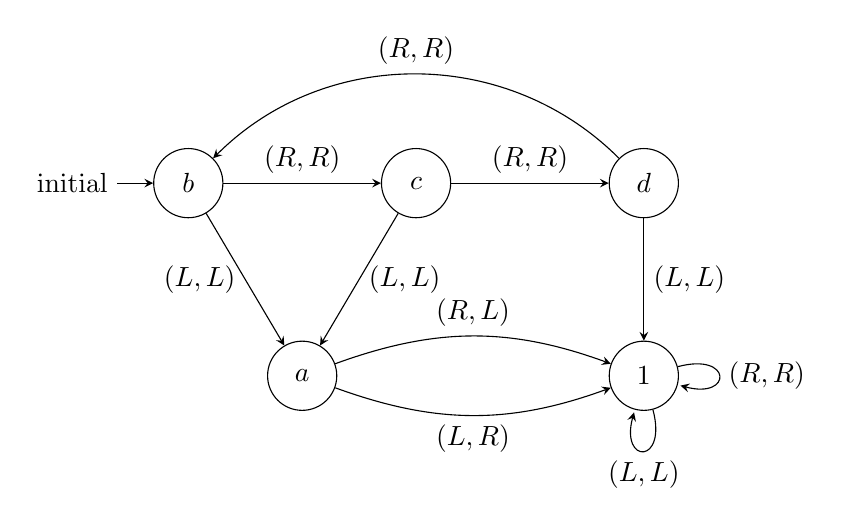
\begin{tikzpicture}[>=stealth,node distance=2,initial text={initial}]

\node [state,initial] (b) {$b$};

\node [state] (c) [right=of b] {$c$};
\node [state] (d) [right=of c] {$d$};
\node [state] (a) [below=of $(b)!0.5!(c)$] {$a$};
\node [state] (1) [below=of $(c)!1!(d)$] {$1$};

\path [->]
	(b)
		edge node [above] {$(R,R)$} (c)
		edge node [left] {$(L,L)$} (a)
	(c)
		edge node [above] {$(R,R)$} (d)
		edge node [right] {$(L,L)$} (a)
	(d)
		edge [bend right=45] node [above] {$(R,R)$} (b)
		edge node [right] {$(L,L)$} (1)
	(a)
		edge [bend left=20] node [above] {$(R,L)$} (1)
		edge [bend right=20] node [below] {$(L,R)$} (1)
	(1)
		edge [loop right] node [right] {$(R,R)$} ()
		edge [loop below] node [below] {$(L,L)$} ()
;

\end{tikzpicture}
\end{document}
